\documentclass[10pt]{elegantbook}

\title{Large Language Model}
\subtitle{Can J.A.R.V.I.S becomes reality?}

\author{occupymars}
\date{June. 23, 2025}
\version{0.1}

\cover{iron_man.jpg}

% all the packages included
\usepackage{cprotect}
\usepackage{fontawesome}
\usepackage[linesnumbered, ruled]{algorithm2e}
\RestyleAlgo{algoruled}

% set some fonts
\setmonofont{Ubuntu Mono}

% my own commands
% \newcommand{\mydefination}[1]{\textit{\textcolor[RGB]{0,174,247}{#1}}}
\newcommand{\mydefination}[1]{\textbf{\textit{\textcolor{structurecolor}{#1}}}}

\begin{document}

\maketitle

\frontmatter
\tableofcontents

\mainmatter

\chapter{Survey}

\section{Large Language Models: A Survey}

\begin{introduction}
    \item Early Pretrained Large Language Models
\end{introduction}

More details please refre to \href{https://arxiv.org/abs/2402.06196}{Large Language Models: A Survey}.

\subsection{Introduction}
Statistical language model are not good because of the data sparsity, early neural language model are task specific.

Large language model have emergent abilities: \mydefination{in-context learning}, where LLMs learn a new task from a small 
set of examples presented in the prompt at inference time; \mydefination{instruction following}, where
LLMs, after instruction tuning, can follow the instructions for new types of tasks without using explicit examples;
\mydefination{multi-step reasoning}, where LLMs can solve a complex task by breaking down that task into intermediate 
reasoning steps.

\begin{figure}[htbp]
    \centering
    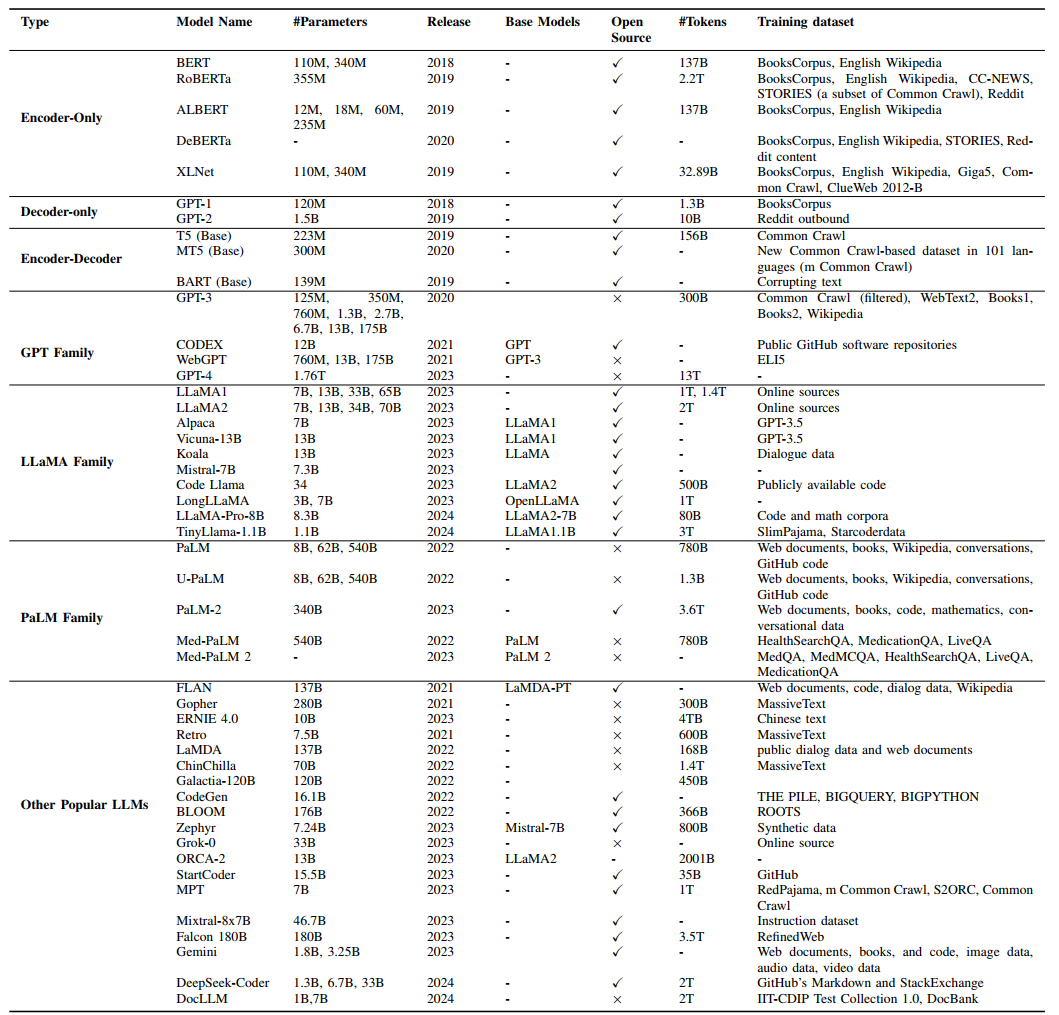
\includegraphics[width=0.90\textwidth]{image/LLM_overview.png}
    \caption{LLM Overview}
    \label{fig:LLM_overview}
\end{figure}

\subsection{Large Language Models}
First let us walk through early pre-trained neural language models. 

\begin{itemize}
    \item The first category is encoder-only models, represented by BERT.
    \begin{enumerate}
        \item BERT, pre-trained by two tasks: \mydefination{masked language modeling} (MLM) and \mydefination{next sentence
    prediction} (NSP)
        \item RoBERTa, remove NSP, train with much larger mini-batches and learning rates.
        \item ALBERT, from $V \times H$ to $V \times E \rightarrow E \times H$ by adding a linear layer, so the embedding layer 
    will has a smaller param size. 24 layers are shared (but the computation speed is same). And new NSP, instead of randomly 
    choose next sequence, inverse the true sequence pair order.
        \item DeBERTa (Decodingenhanced BERT with disentangled attention), use \mydefination{disentangled attention} compute 
    the content and position seperately; At fine-tune stage, add absolute position into decoding layer to predict masked tokens,
    enhance the MLM; Introduce a novel pre-training task, ELECTRA, known as \mydefination{replace token detection} (RTD), instead
    of mask the word, we replace it with plausible alternatives sampled from a small generated model. And pre-training will try
    to distinguish whether tokens are replaced or not. RTD is more sample-efficient than MLM because the former
    is defined over all input tokens rather than just the small subset being masked out.
        \item XLMs, 3 pre-training method, casual language model (CLM) for warmup and basic ability; MLM, shared BPE between
    different language; Translation Language Modeling (TLM), [CLS] ENGLISH [SEP] FRANCH [SEP] with mask.
        \item XLNet, based on Transformer-XL, utilize auto-regressive (decoder), use PLM (permutation language model) to 
    permutate the tokens of a sequence, use AR to predict it (only predict last $K$ tokens) so it can get bidirection information,
    then use a two stream attention because PLM make the position a problem to handle.
        \item UNILM, shared Transformer but three pre-training method, AR, AE (encoder only), seq2seq (encoder-decoder), using 
    different masks to control the context the prediction is conditioned on.
    \end{enumerate}

    \item Second category is decoder-only models, represented by GPT.
    \begin{enumerate}
        \item GPT-1, next token prediction
        \item GPT-2, Layer normalization is moved to the input of each sub-block, additional layer normalization is added
after the final self-attetion block.
    \end{enumerate}

    \item Last category is encoder-decoder PLMs, represented by T5.
    \begin{enumerate}
        \item T5 and mT5 (multilingual variance of T5).
        \item MASS (MAsked Sequence to Sequence pre-training), mask several consecutive tokens as input, decoder predicts
the masked fragment, so it jointly trains language embedding and generation.
        \item BART, it is pre-trained by corrupting text with an arbitrary noising function, and then learning to reconstruct
the original text.
    \end{enumerate}
\end{itemize}

Then we comes to LLM family.
\begin{itemize}
    \item GPT Family
    \begin{enumerate}
        \item GPT-3, maybe the first LLM, with 175B parameters, the first to show in-context learning ability (one of the emergent ability).
        \item CODEX, based on GPT-3, fine-tuned on GitHub, powers Copilot.
        \item WebGPT, based on GPT-3, 3 steps fine-tuned to answer open-ended questions using a text-based web browser (mimic the human, reward, reinforce).
        \item InstructGPT, SFT on labeler-written prompt and demostrations, then further with human-ranked model ouputs build a reinforcement learning flow.
        \item ChatGPT, sibling (brother) model to InstructGPT, the \textcolor{red}{Milestone}.
        \item GPT-4, larger, multimodal input.
    \end{enumerate}

    \item LLaMA
    \begin{enumerate}
        \item LLaMA-1, use the transformer architecture of GPT-3, with modifications: use SwiGLU instead of ReLU; use rotary positional embeddings instead 
    of absolute one; use RMS layer normalization instead of standard one; 13B are better than GPT-3 175B.
        \item LLaMA-2, pre-train -> SFT -> RLFH, last step use accumulation of human feedback for revising the reward model (instead of a big change at short
    time) to save the ability of the model.
        \item Alpaca, first human create 175 instructions, then use pre-trained model to generate other instructions, then generate outputs, clean up, use as
    the SFT data, so this is efficient.
        \item Vicuna-13B, fine-tuned on user-shared conversations from ShareGPT.
        \item Guanaco, use \mydefination{QLoRA} to fine-tune, back-propagates gradients through a frozen, 4-bit quantized pre-trained language model into Low Rank Adapters.
        \item Koala fine-tuned with data from ChatGPT.
        \item Mistral-7B leverages grouped-query attention for faster inference, sliding window attention to efficiently handle sequences of arbitrary length.
    Better than most 13B and 34B model at that time.
    \end{enumerate}

    \item PaLM (Pathways [a distrubuted system] Language Model)
    \begin{enumerate}
        \item PaLM is a 540B model.
        \item U-PaLM trained with UL2R (Unified Language Learner with Residual Learning), first learn simple task (80\% are simple tasks), then learn complicated
    one, use mixture-of-denoiser objective.
        \item Flan-PaLM is fine-tuned U-PaLM with instrunction. Large SFT datasets, 473 datasets with 146 categories.
        \item PaLM-2 is efficient and multilingual model.
        \item Med-PaLM, use \mydefination{instruction prompt tunning}, add a soft prompt at the embedding, and learn it (the model is frozen). So the method is
    more efficient than adapter method like LoRA, and it preformance is better than hard prompting.
    \end{enumerate}

    \item Other LLMs
    \begin{enumerate}
        \item FLAN, shows that \mydefination{instruction fine-tune} is good for zero-shot and multi-shot preformance, inspires ChatGPT instruction align tech and prompt engineer.
        \item Gopher, analysis of model scales on model preformance.
        \item T0, extend of FLAN, multi-prompt training.
        \item ERNIE 3.0, combine AR and AE. Injection of knowledge graph.
        \item RETRO, milestone of \mydefination{Retrieval-Augmented Generation}, with a similarity based chunk cross attention.
        \item GLaM, \mydefination{Mixture-of-experts} (MOE), replace the FFN layer with Gated FFN, which will choose different sub-layer using the gate, 
    less training computation and inference computation.
        \item LaMDA, trained on dialog data, focus on safety.
        \item OPT
        \item Chinchilla, limite the compute budget, train different size of model and dateset, find that these two size should be sacled equally.
        \item Galactica, trained on scientific corpus.
        \item CodeGen, conversational programming (multi-step programming).
        \item AlexaTM, mixture of denoising and CLM tasks, more efficient few-shot learners thant decoder-only models on various tasks. Multilingual model.
        \item Sparrow, use RLFH to create harmless, safety dialogue. Two modeling of outputs to help human labeler.
        \item Minerva, math enhanced.
        \item MoD, mixture-of-denoisers as the objectives.
        \item BLOOM, which promotes transparent, collaborative AI research.
        \item GLM, english-chinese model.
        \item Pythia, trained on public data in a consistent sequence, with 154 checkpoints per model. It enables research on LLM training dynamics, 
    memorization, term frequency effects, and gender bias reduction.
        \item Orca, imitation learning, teacher assistance from ChatGPT.
        \item StarCoder, 80+ programming languages.
        \item KOSMOS, advancing research in cross-modal AI applications.
    \end{enumerate}
\end{itemize}

\subsection{How LLMs are built}
\begin{figure}[htbp]
    \centering
    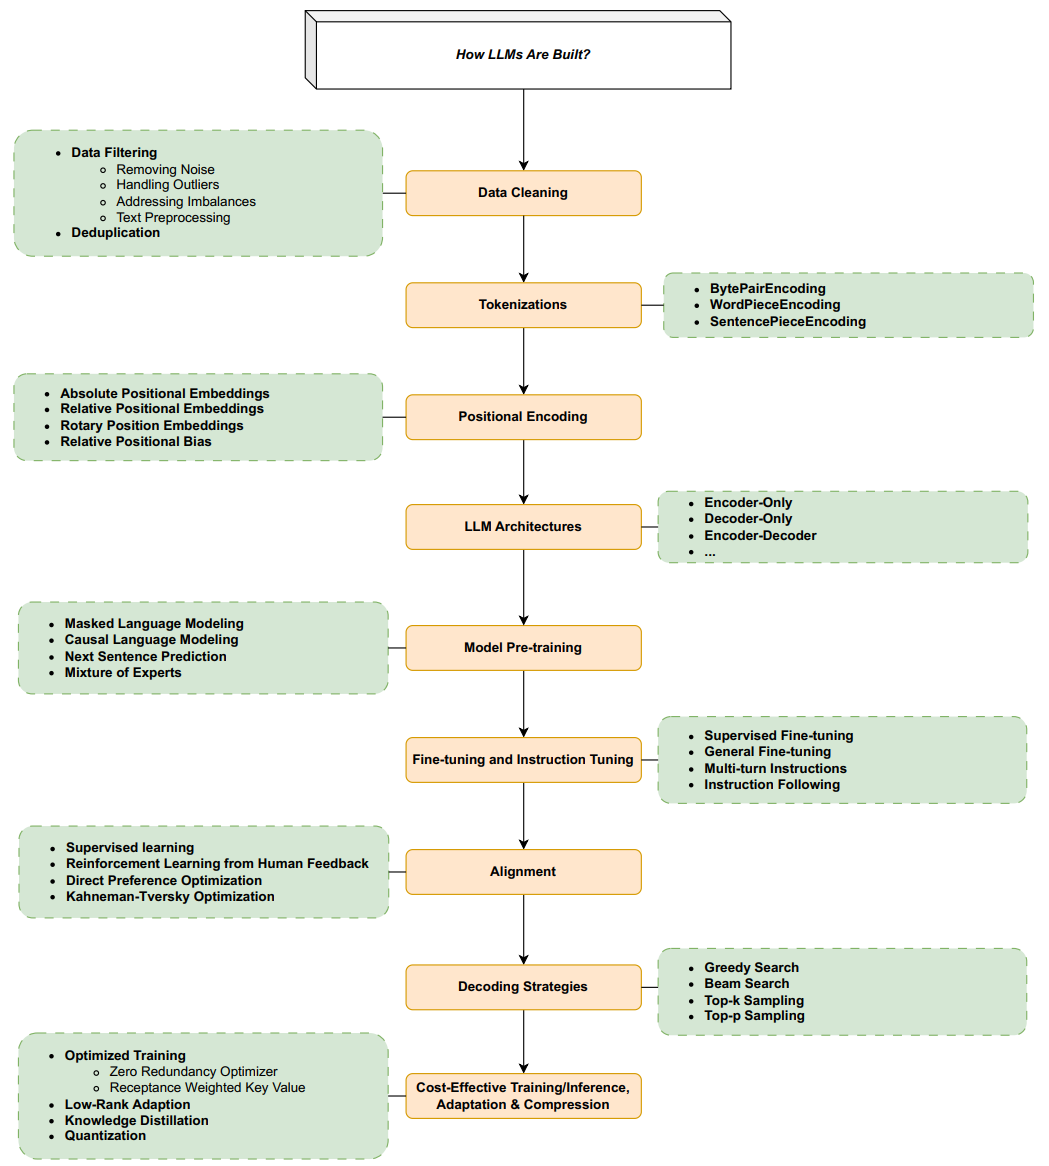
\includegraphics[width=0.90\textwidth]{image/how_llm_works.png}
    \caption{Components of LLMs}
    \label{fig:how_llm_works}
\end{figure}

\chapter{History Language Models}

\section{Statistical Language Model}

\mydefination{N-Gram} model is the most dominating form of SLMs, which is a Markov chain model, using the statistic from
previous $n-1$ words and current word.
\[ P(w_n \mid w_{n-k}, \ldots, w_{n-1}) = \frac{count(w_{n-k}, \ldots, w_{n})}{count(w_{n-k}, \ldots, w_{n-1})} \]
in n-gram, $k$ is always $n-1$.

In order to deal with unseen words and small probability of larger n-pairs, smooth method are often used, like 
\mydefination{Laplace-smooth}.

\end{document}